\chapter{Implementación}

En esta sección vamos a tratar como se ha implementado el proyecto sobre el cual se basa esta memoria y sus principales módulos.Contiene 3 secciones. La primera llamada Hito 1: Asistente entrenamiento potencia 7.1, describe los pasos realizados para implementar el ecosistema de la aplicación móvil. La segunda, denominada Hito 2: Uso del servidor, describe los pasos realizados para implementar la conexión con el servidor. Finalmente, la sección Capturas 7.3, contiene capturas sobre la aplicación.
\\
\\

La arquitectura del proyecto sigue el siguiente esquema, el cual se ha desarrollado a lo largo de las dos historias de usuario:

\begin{figure}[H]
	\centering
	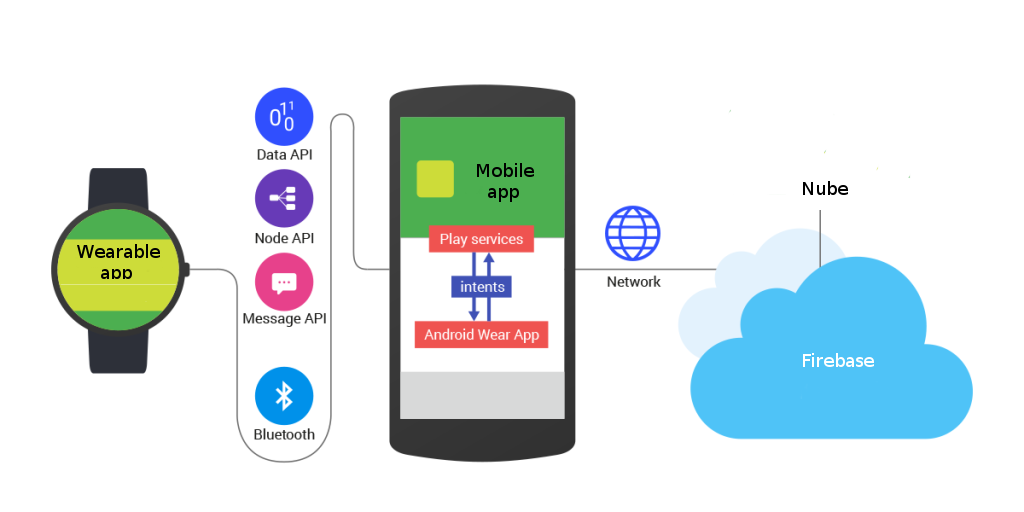
\includegraphics[scale=0.4]{imagenes/arquitectura.png}
	\caption{Diagrama de clases de la aplicación móvil.}
	\label{Arquitectura del sistema}
\end{figure}

El proyecto ha sido desarrollado en Android, por lo que la parte lógica ha sido totalmente programada en Java y utiliza XML para crear las distintas vistas.

\section{Hito 1: Asistente entrenamiento potencia}


El primer paso fue la creación de dos aplicaciones básicas, las cuales incluían una actividad MainActivity, sin ninguna funcionalidad. Una vez creadas ambas aplicaciones había que establecer un cauce de comunicación entre ambas aplicaciones, para ello se ha utilizado la API GoogleApiClient.
\\
Debemos tener en cuenta de que para realizar la conexión, debe haberse instalado previamente la aplicación Android Wear y debe estar enlazada al smartwatch que deseemos usar. Una vez hemos creado una instancia de GoogleApiClient, debemos conectar a la API Wearable API. Se debe establecer la conexión tanto en la aplicación wear como en la móvil para crear el cauce de comunicación.
\\
\\
Tras la creación de un cauce de comunicación entre ambas aplicaciones, se procedió a la obtención de los datos de los sensores. Para ello se utilizo la API de Android y el tipo de sensor TYPE\_LINEAR\_ACCELERATION. Que como se pudo ver en el capítulo 5, fue el método que menor error produjo en las muestras.
\\
\\
De manera paralela, se creó una selección de ejercicios disponibles en la aplicación móvil, añadiendo una pequeña descripción a cada ejercicio.
\\
\\
Una vez obtenidos los datos, se procedió al envío de los mismos en la aplicación Wear, haciendo uso del cauce que se había creado previamente. Utilizando la API DataApi, se creó un objeto DataItem, el cual mediante peticiones se utiliza para el envío de datos sincronizados.\\
A su vez, se procedió a la creación de un listener para el DataItem (utilizando también la API DataApi) en la aplicación móvil, de modo que los datos fueran recibidos en la aplicación móvil.
\\
\\
Todo este proceso se realizó sin ningún control del envio y recepción, siendo estos realizados de manera automática. Por lo que tras estos pasos, se procedió a crear una interfaz de control en la aplicación wear para poder iniciar y detener el envío de información. Dando por finalizada la aplicación Wear.
\\
\\
Estando la comunicación establecida y una vez recibidos los datos se procedió al filtrado de los datos por medio de una ventana de discriminación con el fin de eliminar parte del ruido de los datos.
\\
Posteriormente, con los datos procesados, se procedió al cálculo de la velocidad utilizando un algoritmo de integración. Representando la velocidad calculada haciendo uso de la librería GraphView\cite{graphview}. Cuyo código puede ser consultado en la página del desarrollador y se encuentra bajo licencia Apache v2.
\\
\\
Finalmente, se introdujo un campo para que el usuario introduzca el peso con el que va a realizar el ejercicio y con estos datos, se produjo a calcular la potencia obtenida en cada momento por el usuario.
\\
\\
Estando así la funcionalidad principal de la aplicación completa y totalmente operativa. Sin embargo, carecía de una interfaz gráfica que facilitase la experiencia del usuario. Por lo que se procedió a la creación de un menú  en base a Bottom navigation de material design\cite{navigation}. Utilizando fragments para las distintas vistas del menú.

\section{Hito 2: Uso del servidor}

En este hito se centró en ampliar la funcionalidad de la aplicación por medio de un servidor.
\\
\\
El primer paso fue crear un proyecto en la consola de Firebase.
\\
Una vez importado el paquete Firebase en la aplicación móvil, se utilizó la librería auth para la creación de usuarios (previa activación en la consola de Firebase), inicio de sesión y mantenimiento de la sesión.
\\
Para la obtención de credenciales se crearon dos vistas, una para el registro y otra para el inicio de sesión. En las cuales se obtienen los datos del usuario.
\\
\\
Se utiliza la librería database para las operaciones de escritura lectura de la base de datos, siguiendo el esquema que se diseño en la fase de diseño de la base de datos. Escribiendo en la base de datos al realizar el ejercicio y creando una nueva vista para recuperar los datos guardados en la base de datos, utilizando el criterio de la fecha como clave de búsqueda.
\\
\\
Además, cuando el sistema se encuentre sin conexión a la red y se este realizando un ejercicio. El sistema guardará los datos en almacenamiento local, procediendo al envío de los mismos en cuanto se disponga de conexión y liberando así el espacio ocupado.

\section{Capturas}

Tras la finalización de los dos hitos, a continuación se adjuntan capturas de pantalla de la aplicación.

\subsection*{Android Wear}

En la aplicación de Adroid Wear solo contamos con una vista, la cual va cambiando si el usuario quiere comenzar o terminar un ejercicio.

\begin{figure}[H]
	\centering
	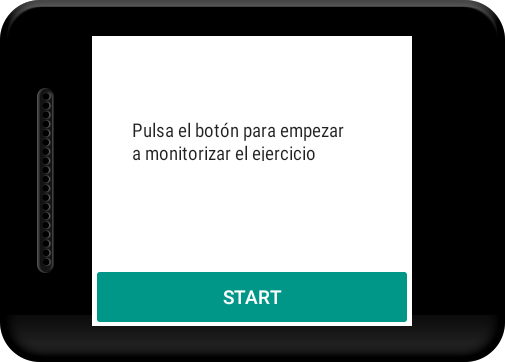
\includegraphics[scale=0.4]{imagenes/w1.png}
	\caption{Pantalla principal Wear}
	\label{Pantalla principal Wear}
\end{figure}

\begin{figure}[H]
	\centering
	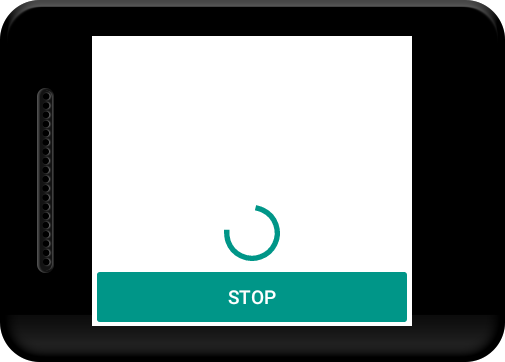
\includegraphics[scale=0.4]{imagenes/w2.png}
	\caption{Realizar medición Wear}
	\label{Realizar medición Wear}
\end{figure}

\subsection*{Android}

Las vistas más importantes de la aplicación móvil son:

\begin{figure}[H]
	\centering
	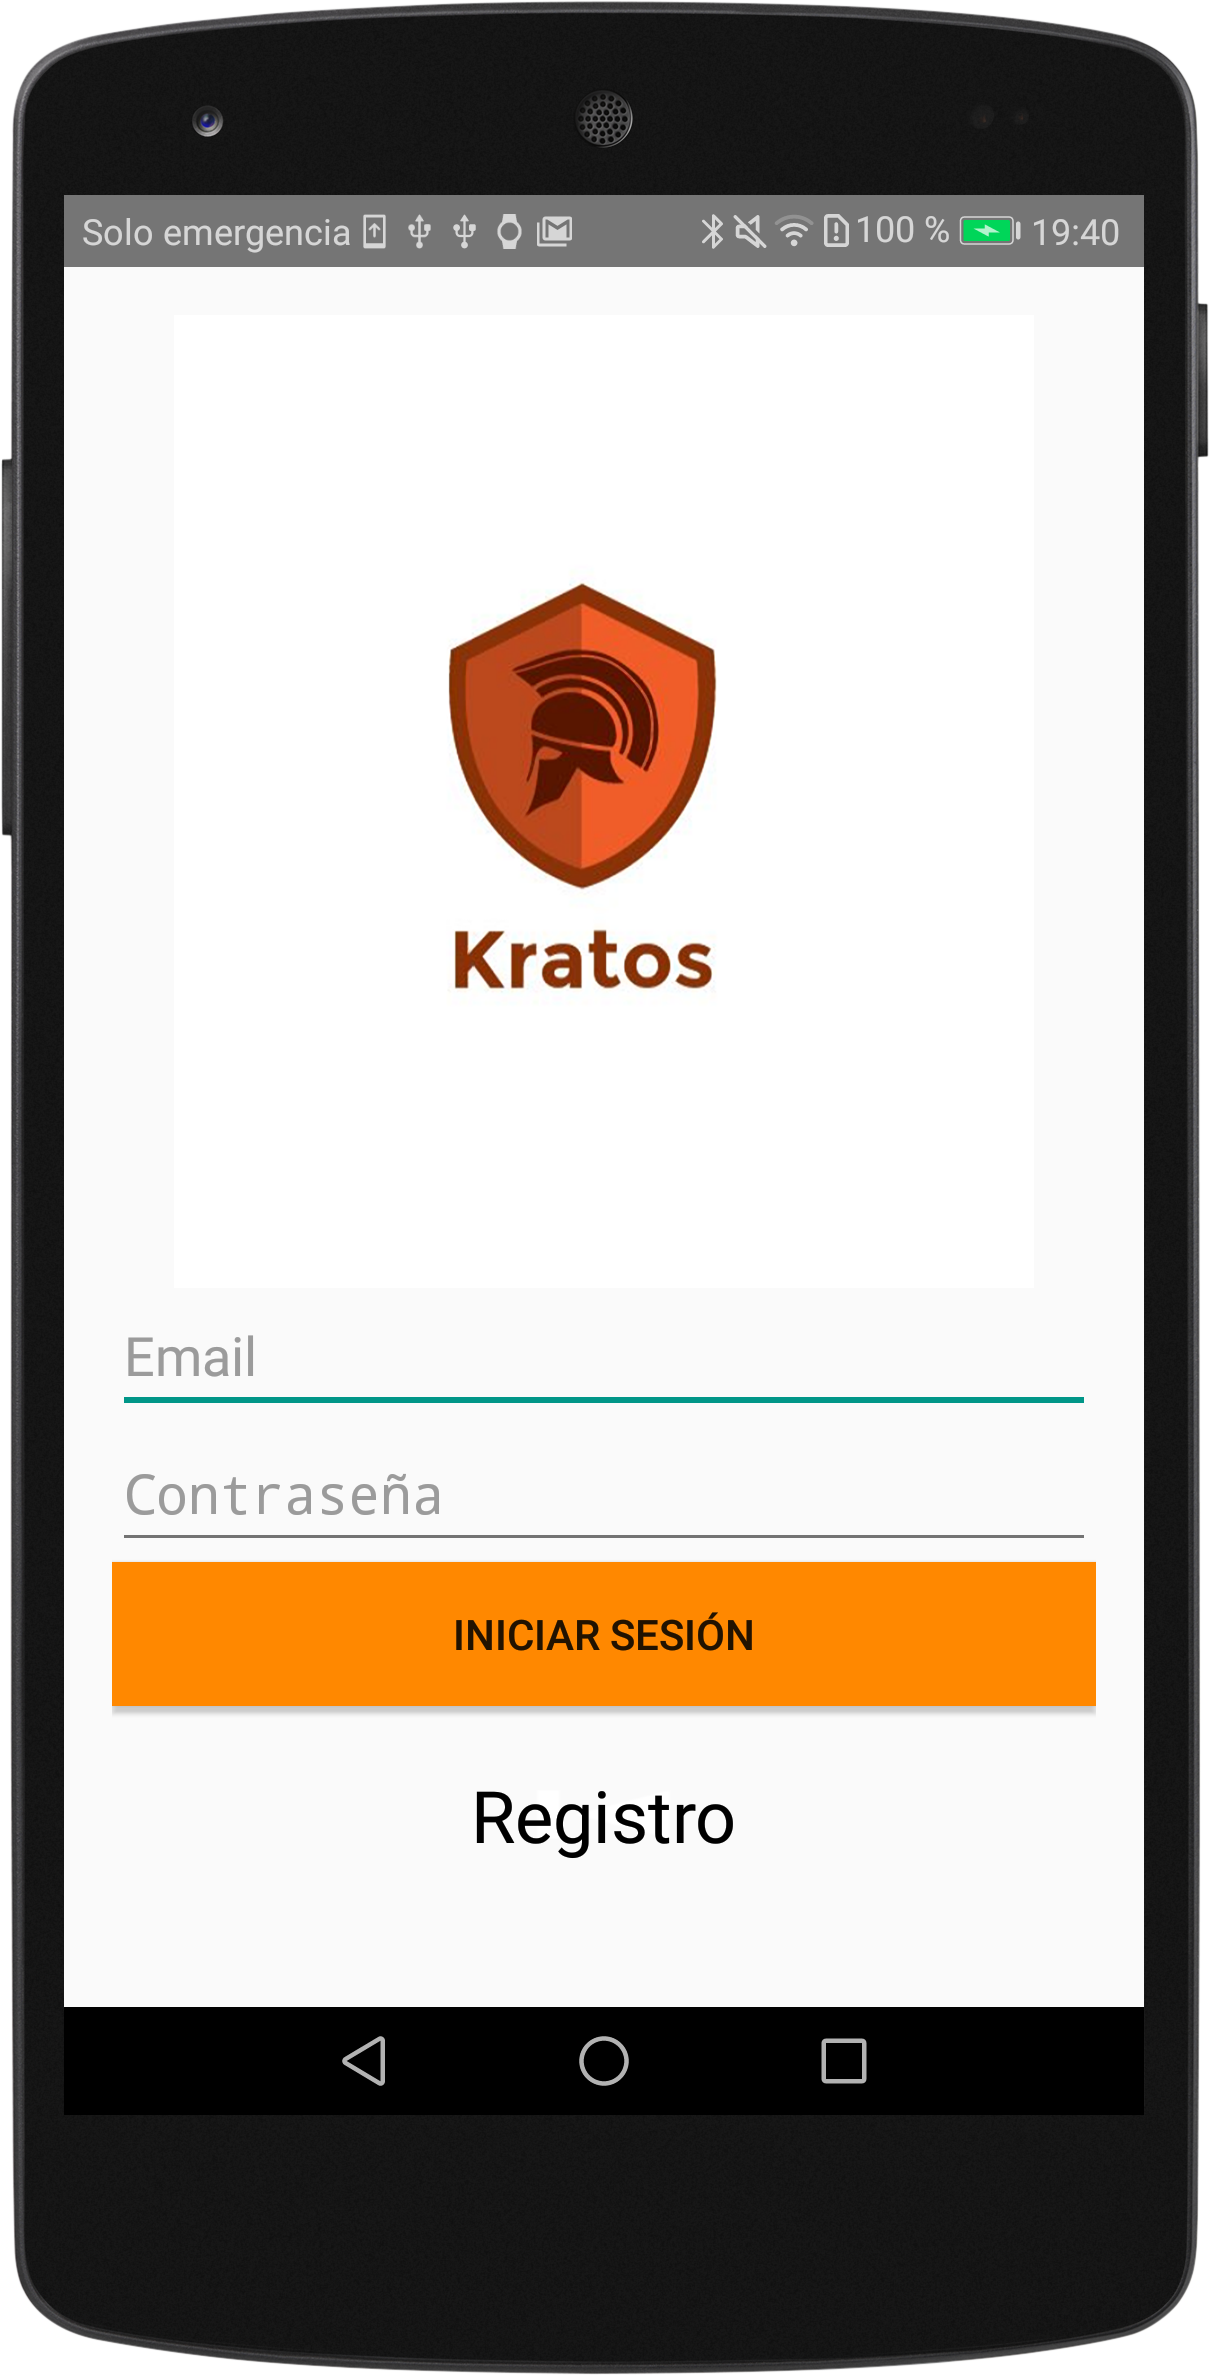
\includegraphics[scale=0.10]{imagenes/m1.png}
	\caption{Pantalla inicio sesión móvil}
	\label{Pantalla inicio sesión móvil}
\end{figure}

\begin{figure}[H]
	\centering
	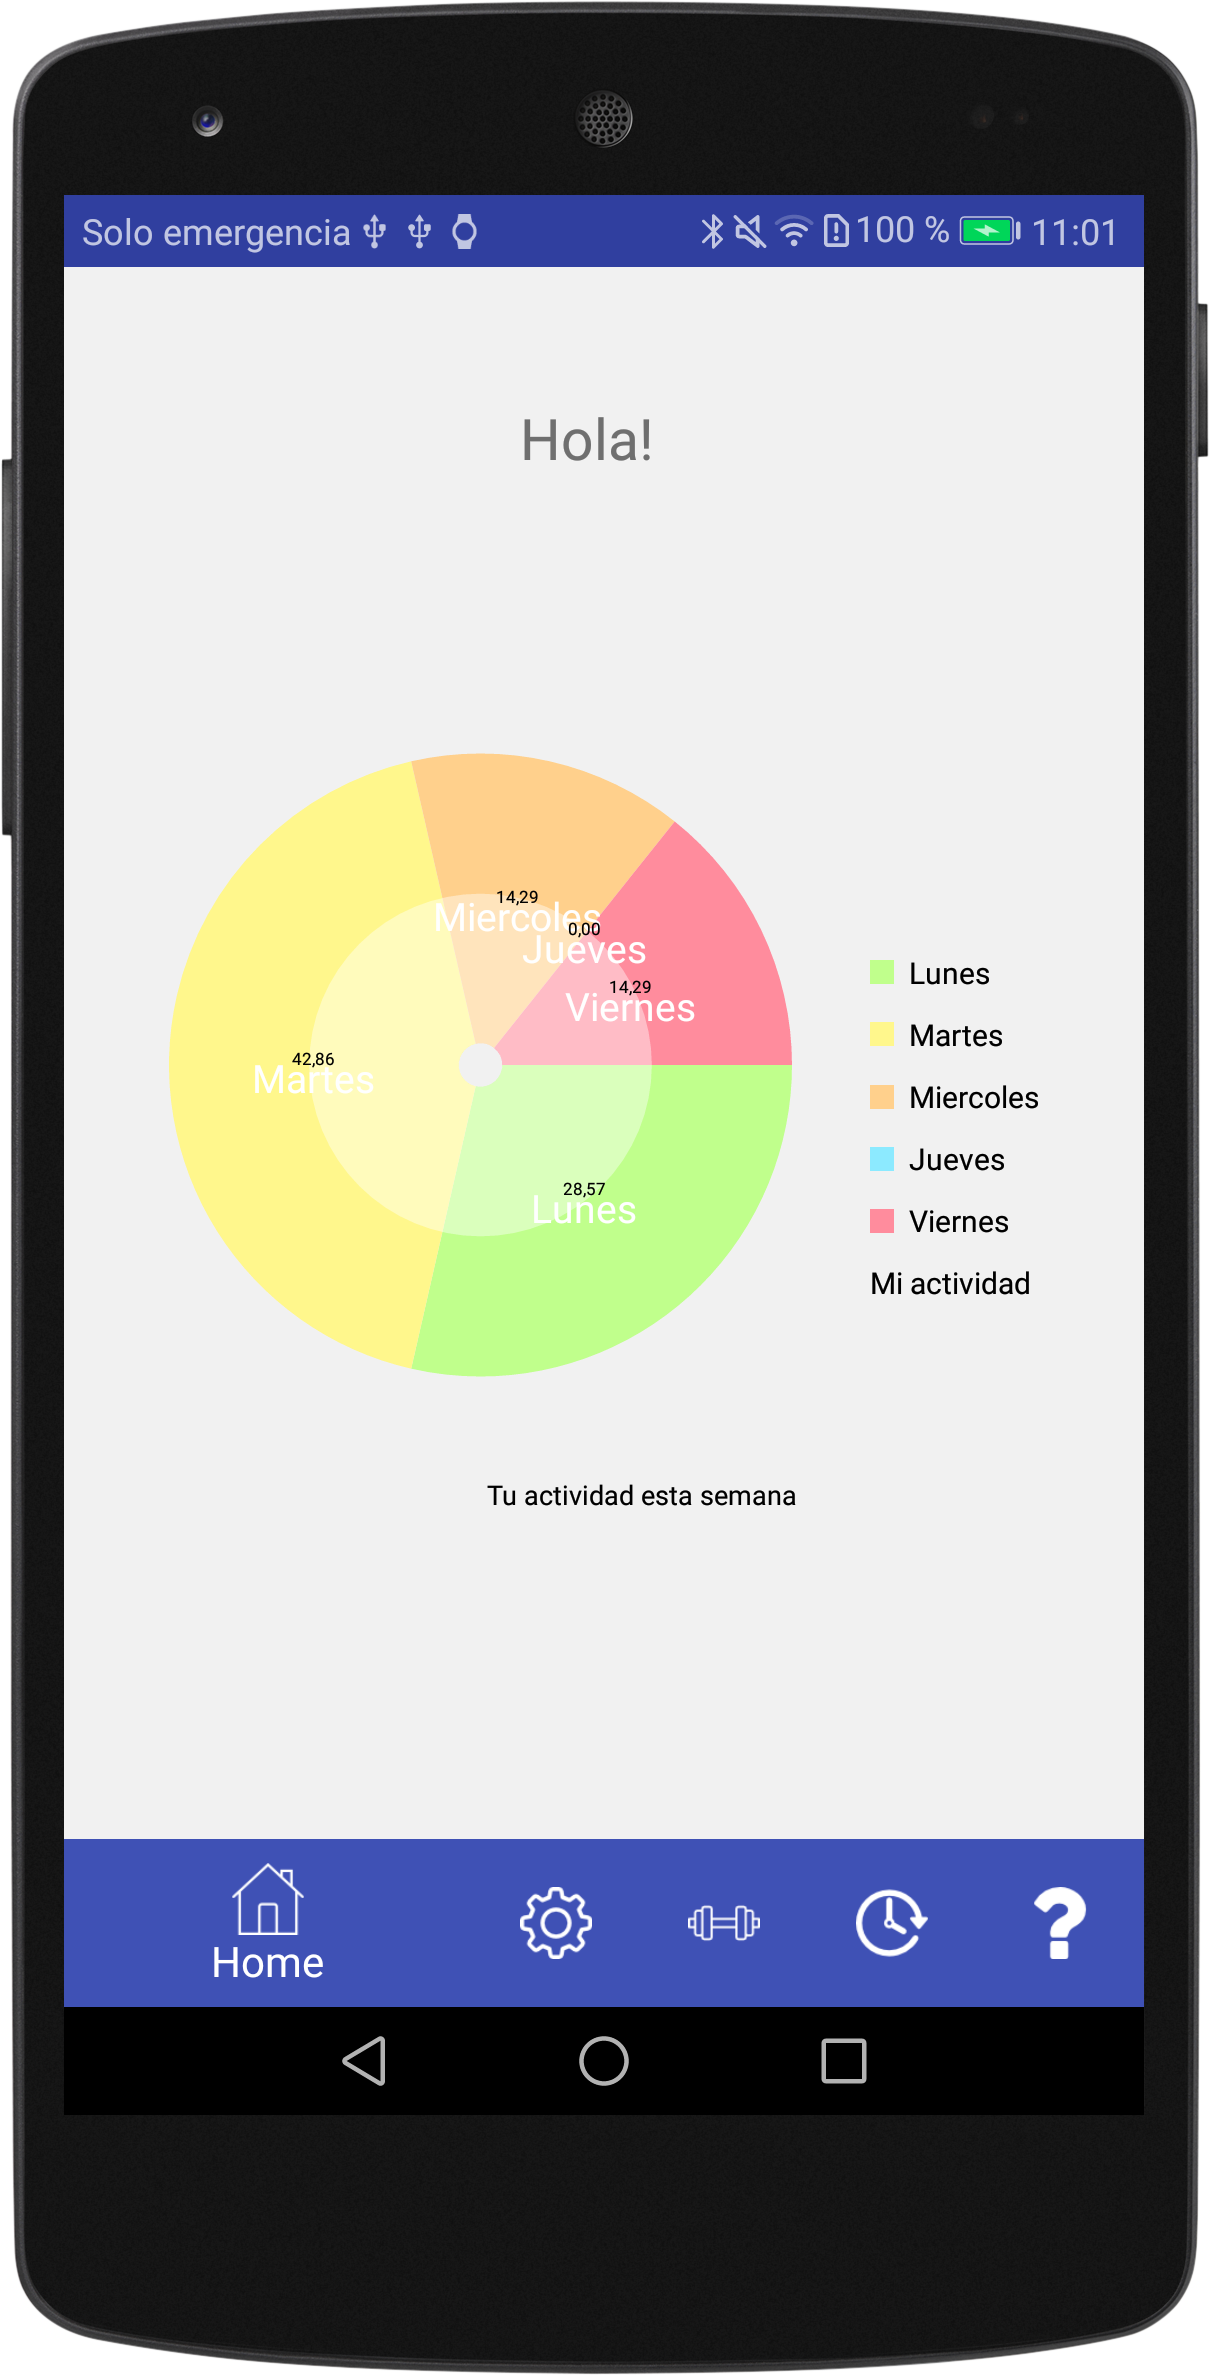
\includegraphics[scale=0.10]{imagenes/m2.png}
	\caption{Pantalla principal móvil}
	\label{Pantalla principal movil}
\end{figure}

\begin{figure}[H]
	\centering
	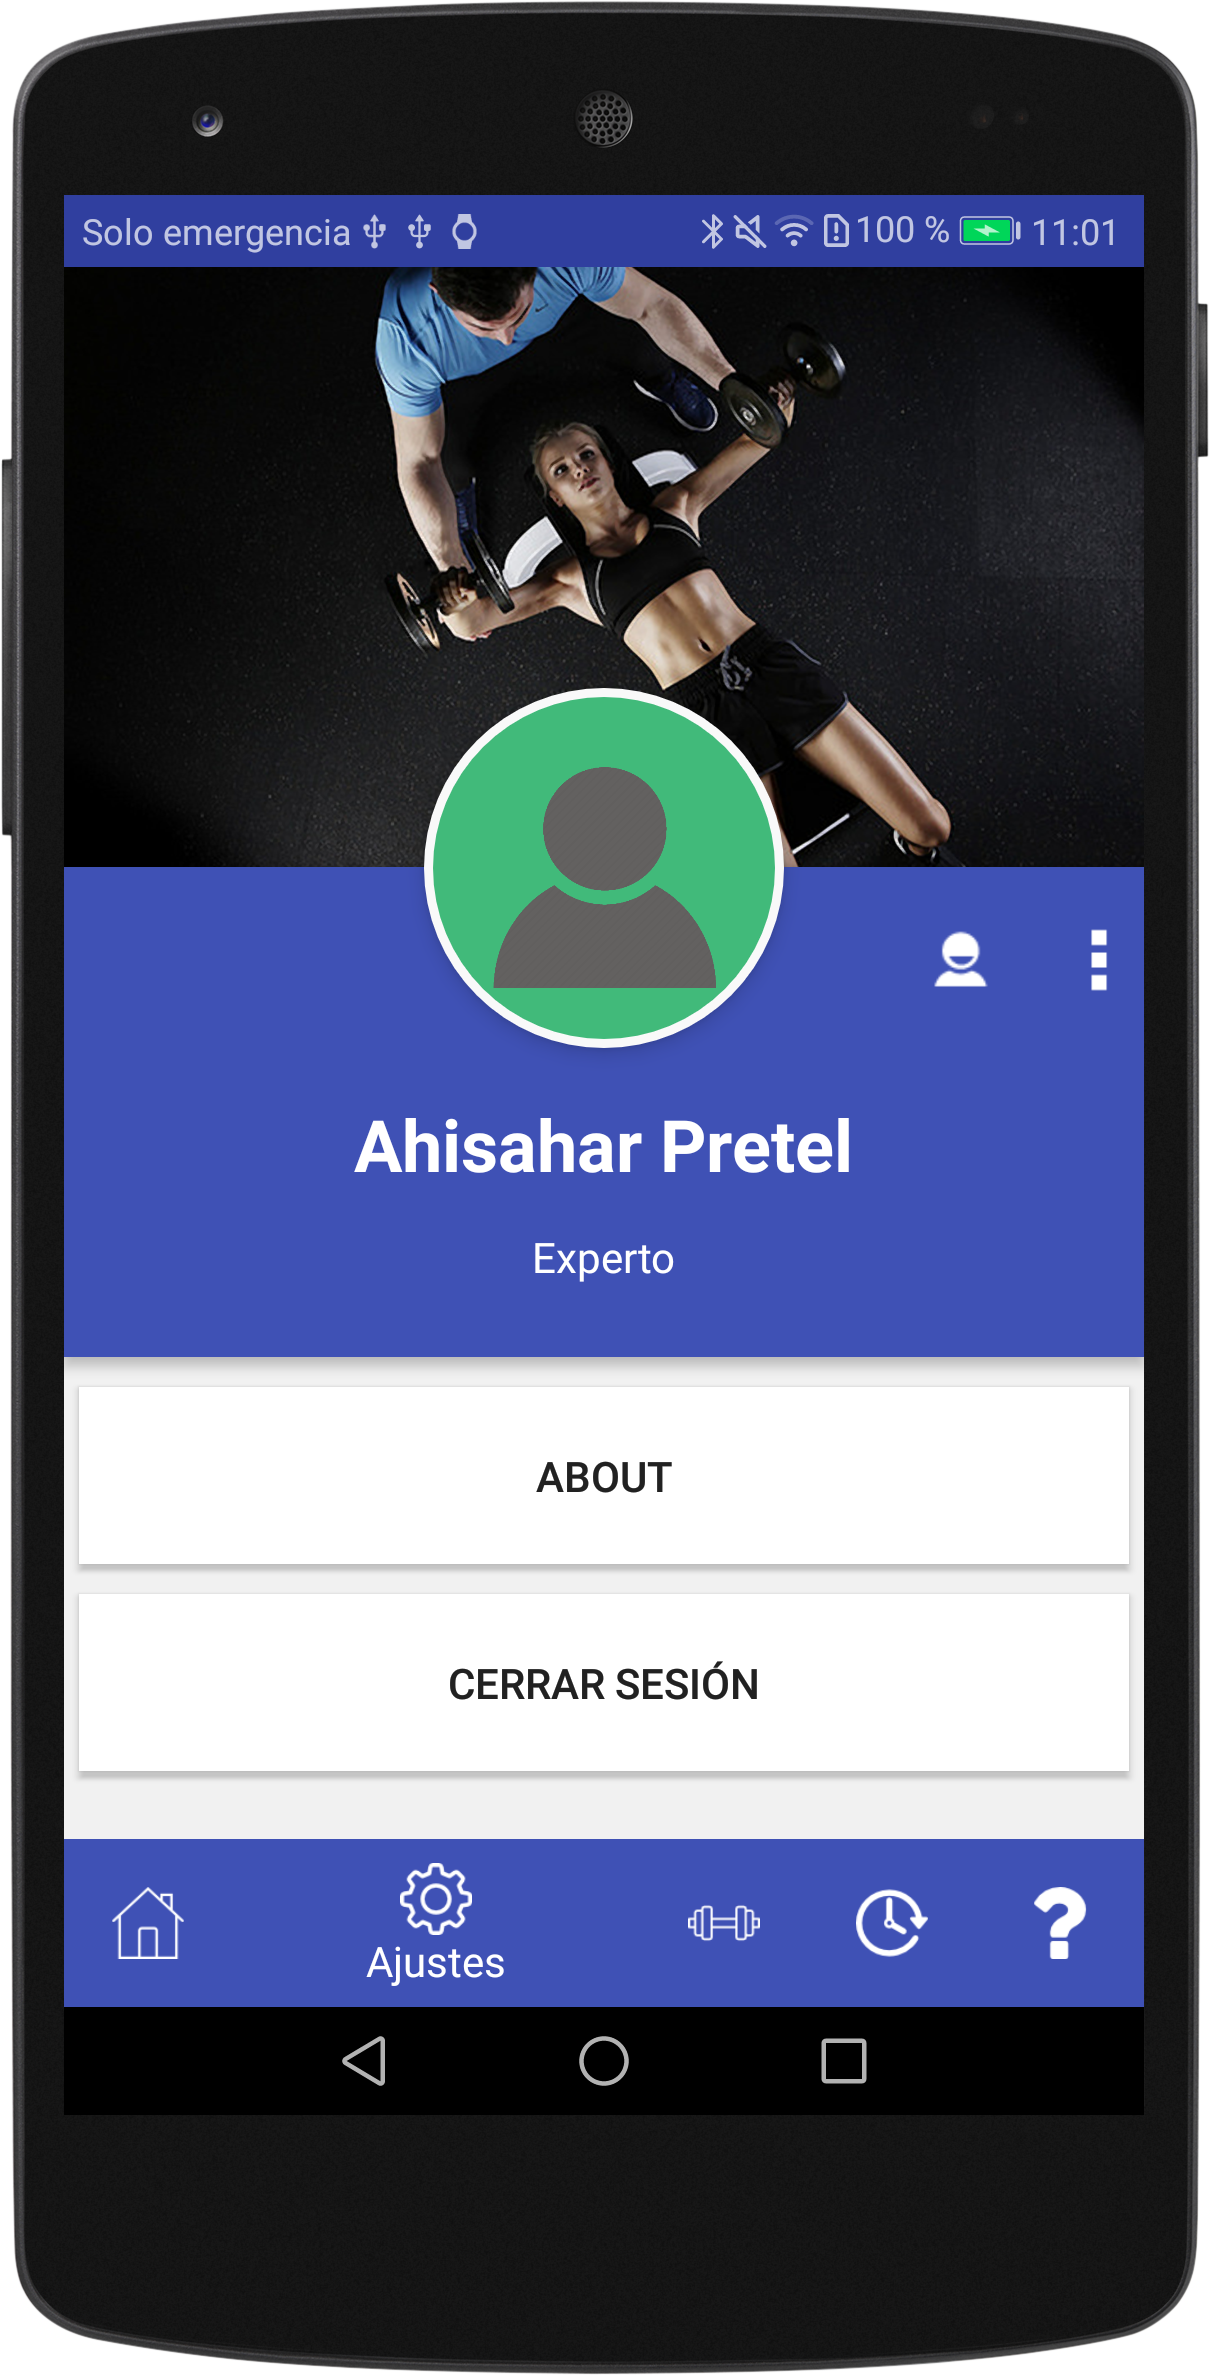
\includegraphics[scale=0.10]{imagenes/m3.png}
	\caption{Vista menú móvil}
	\label{Vista menú movil}
\end{figure}

\begin{figure}[H]
	\centering
	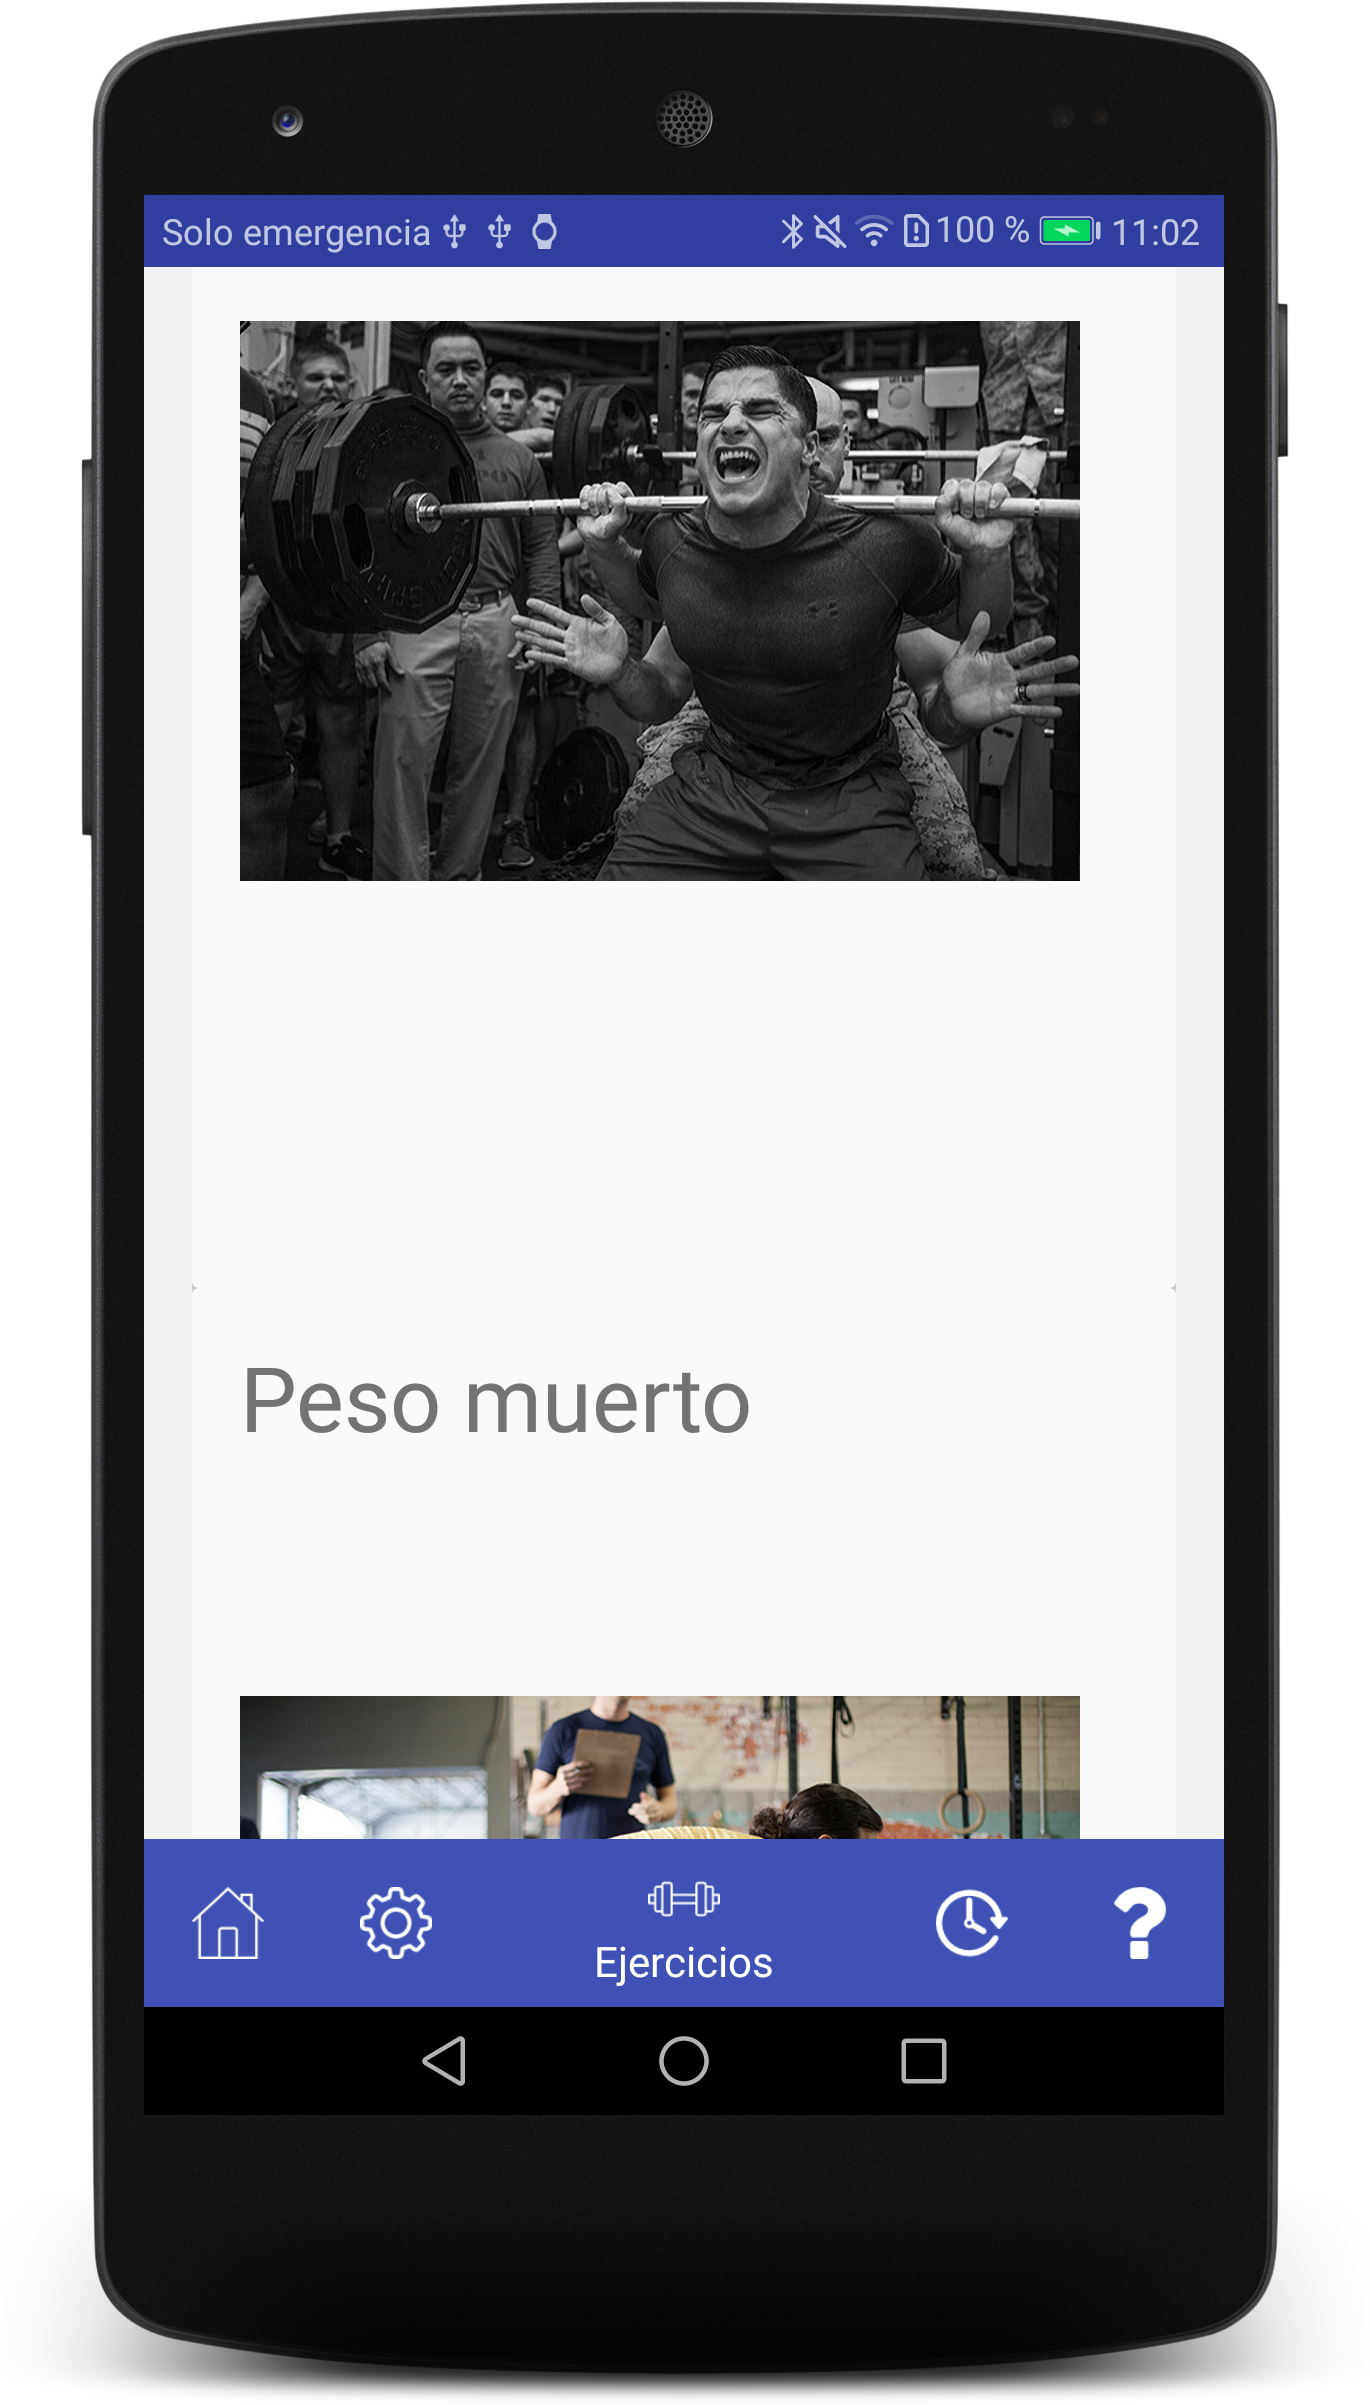
\includegraphics[scale=0.10]{imagenes/m4.png}
	\caption{Vista selección ejercicio móvil}
	\label{Vista selección ejercicio movil}
\end{figure}

\begin{figure}[H]
	\centering
	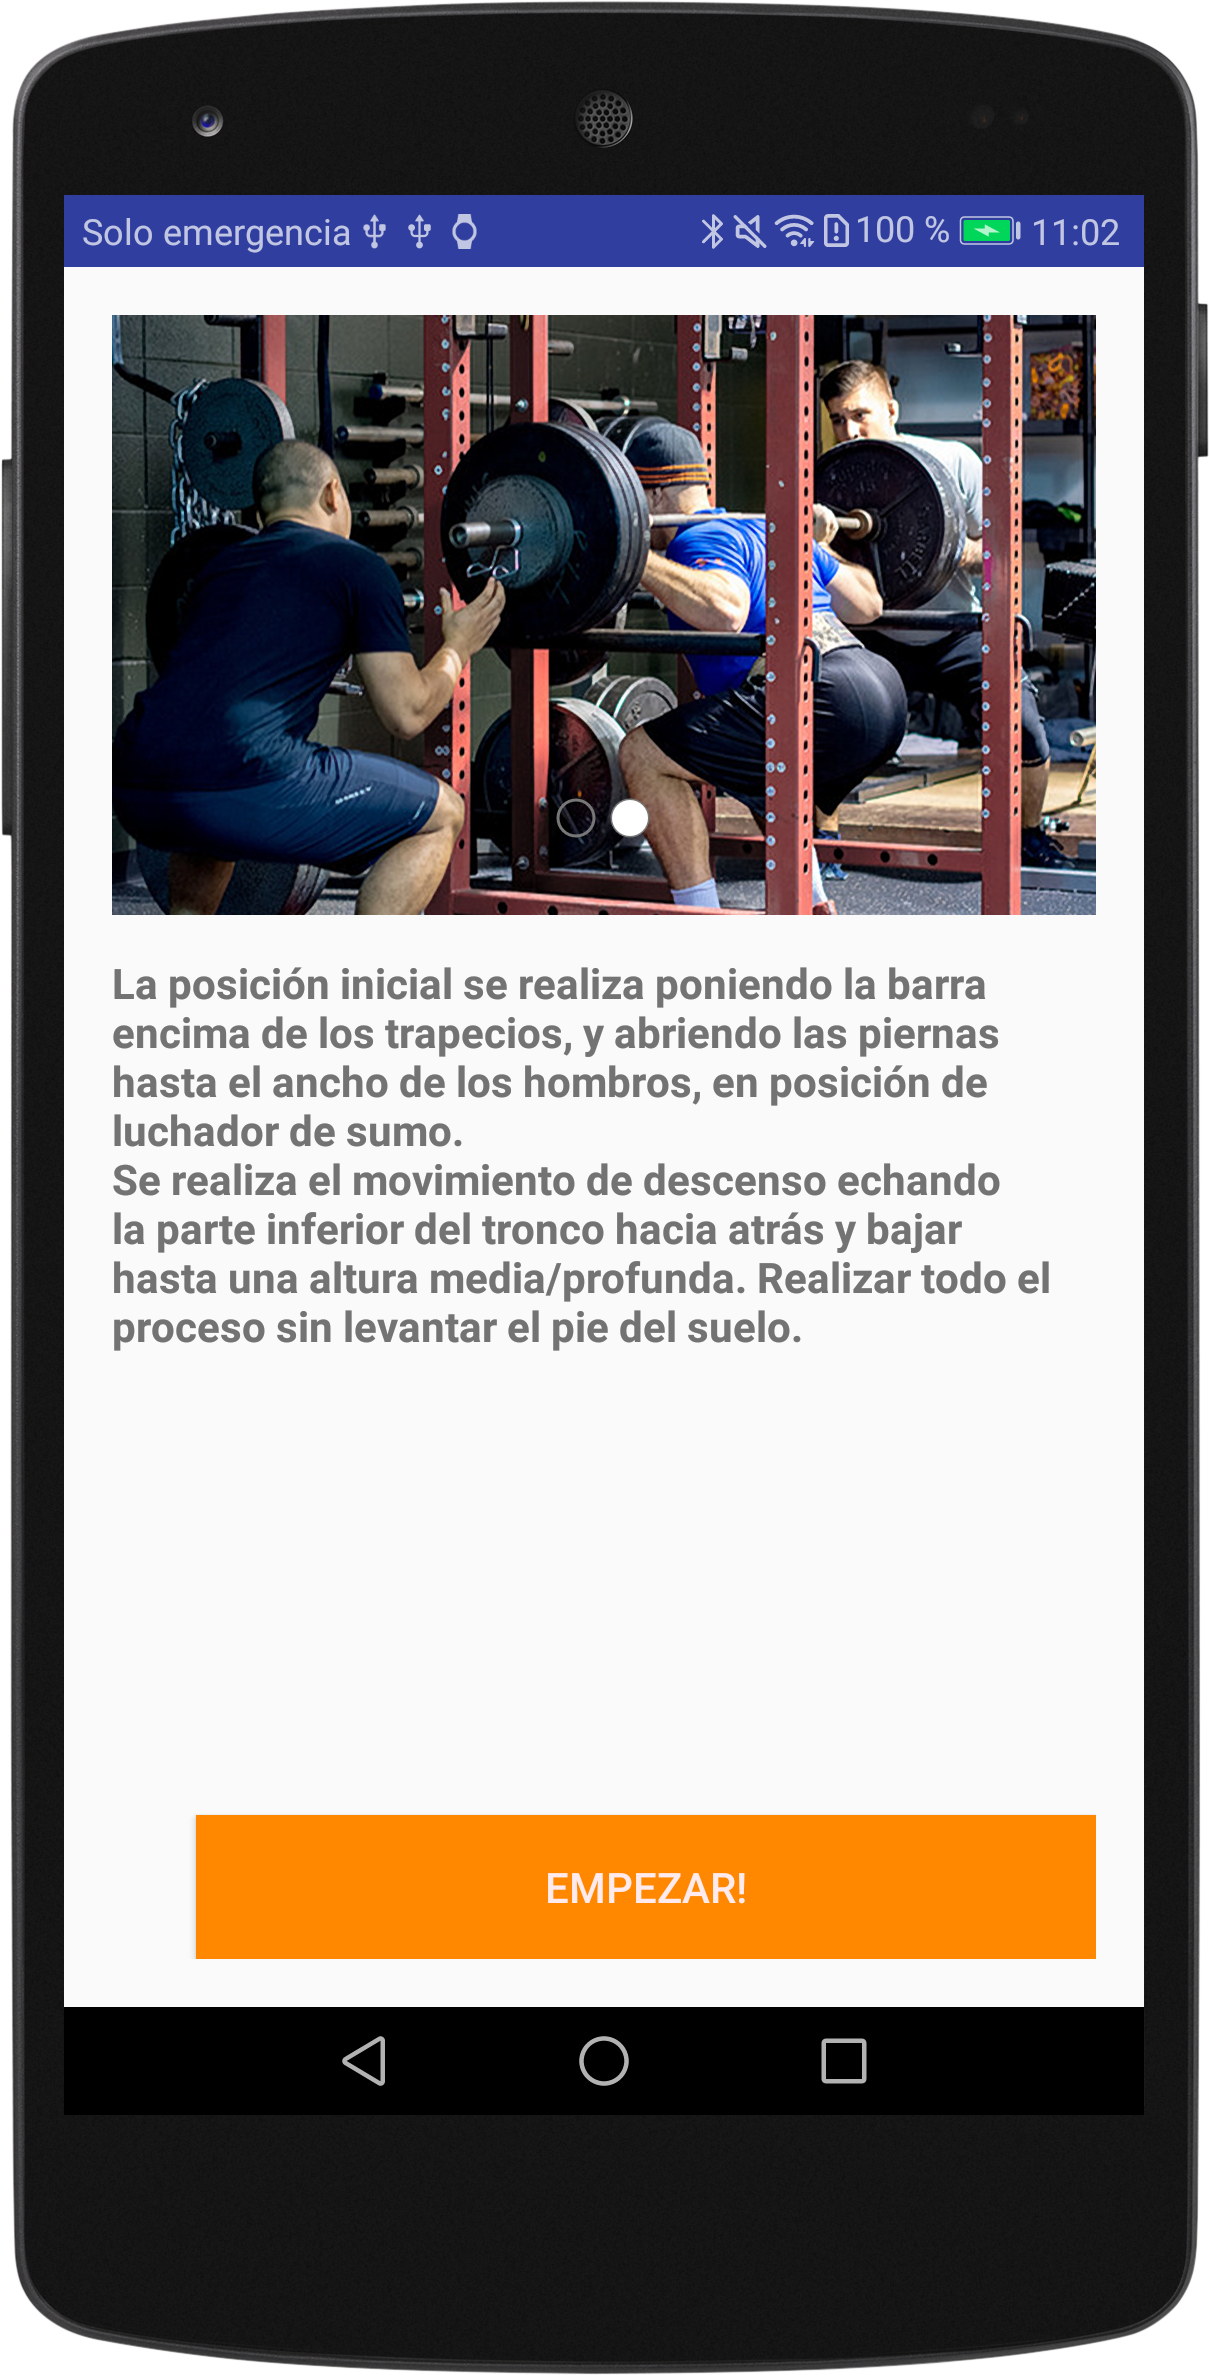
\includegraphics[scale=0.10]{imagenes/m5.png}
	\caption{Vista descripción ejercicio móvil}
	\label{Vista descripción ejercicio movil}
\end{figure}

\begin{figure}[H]
	\centering
	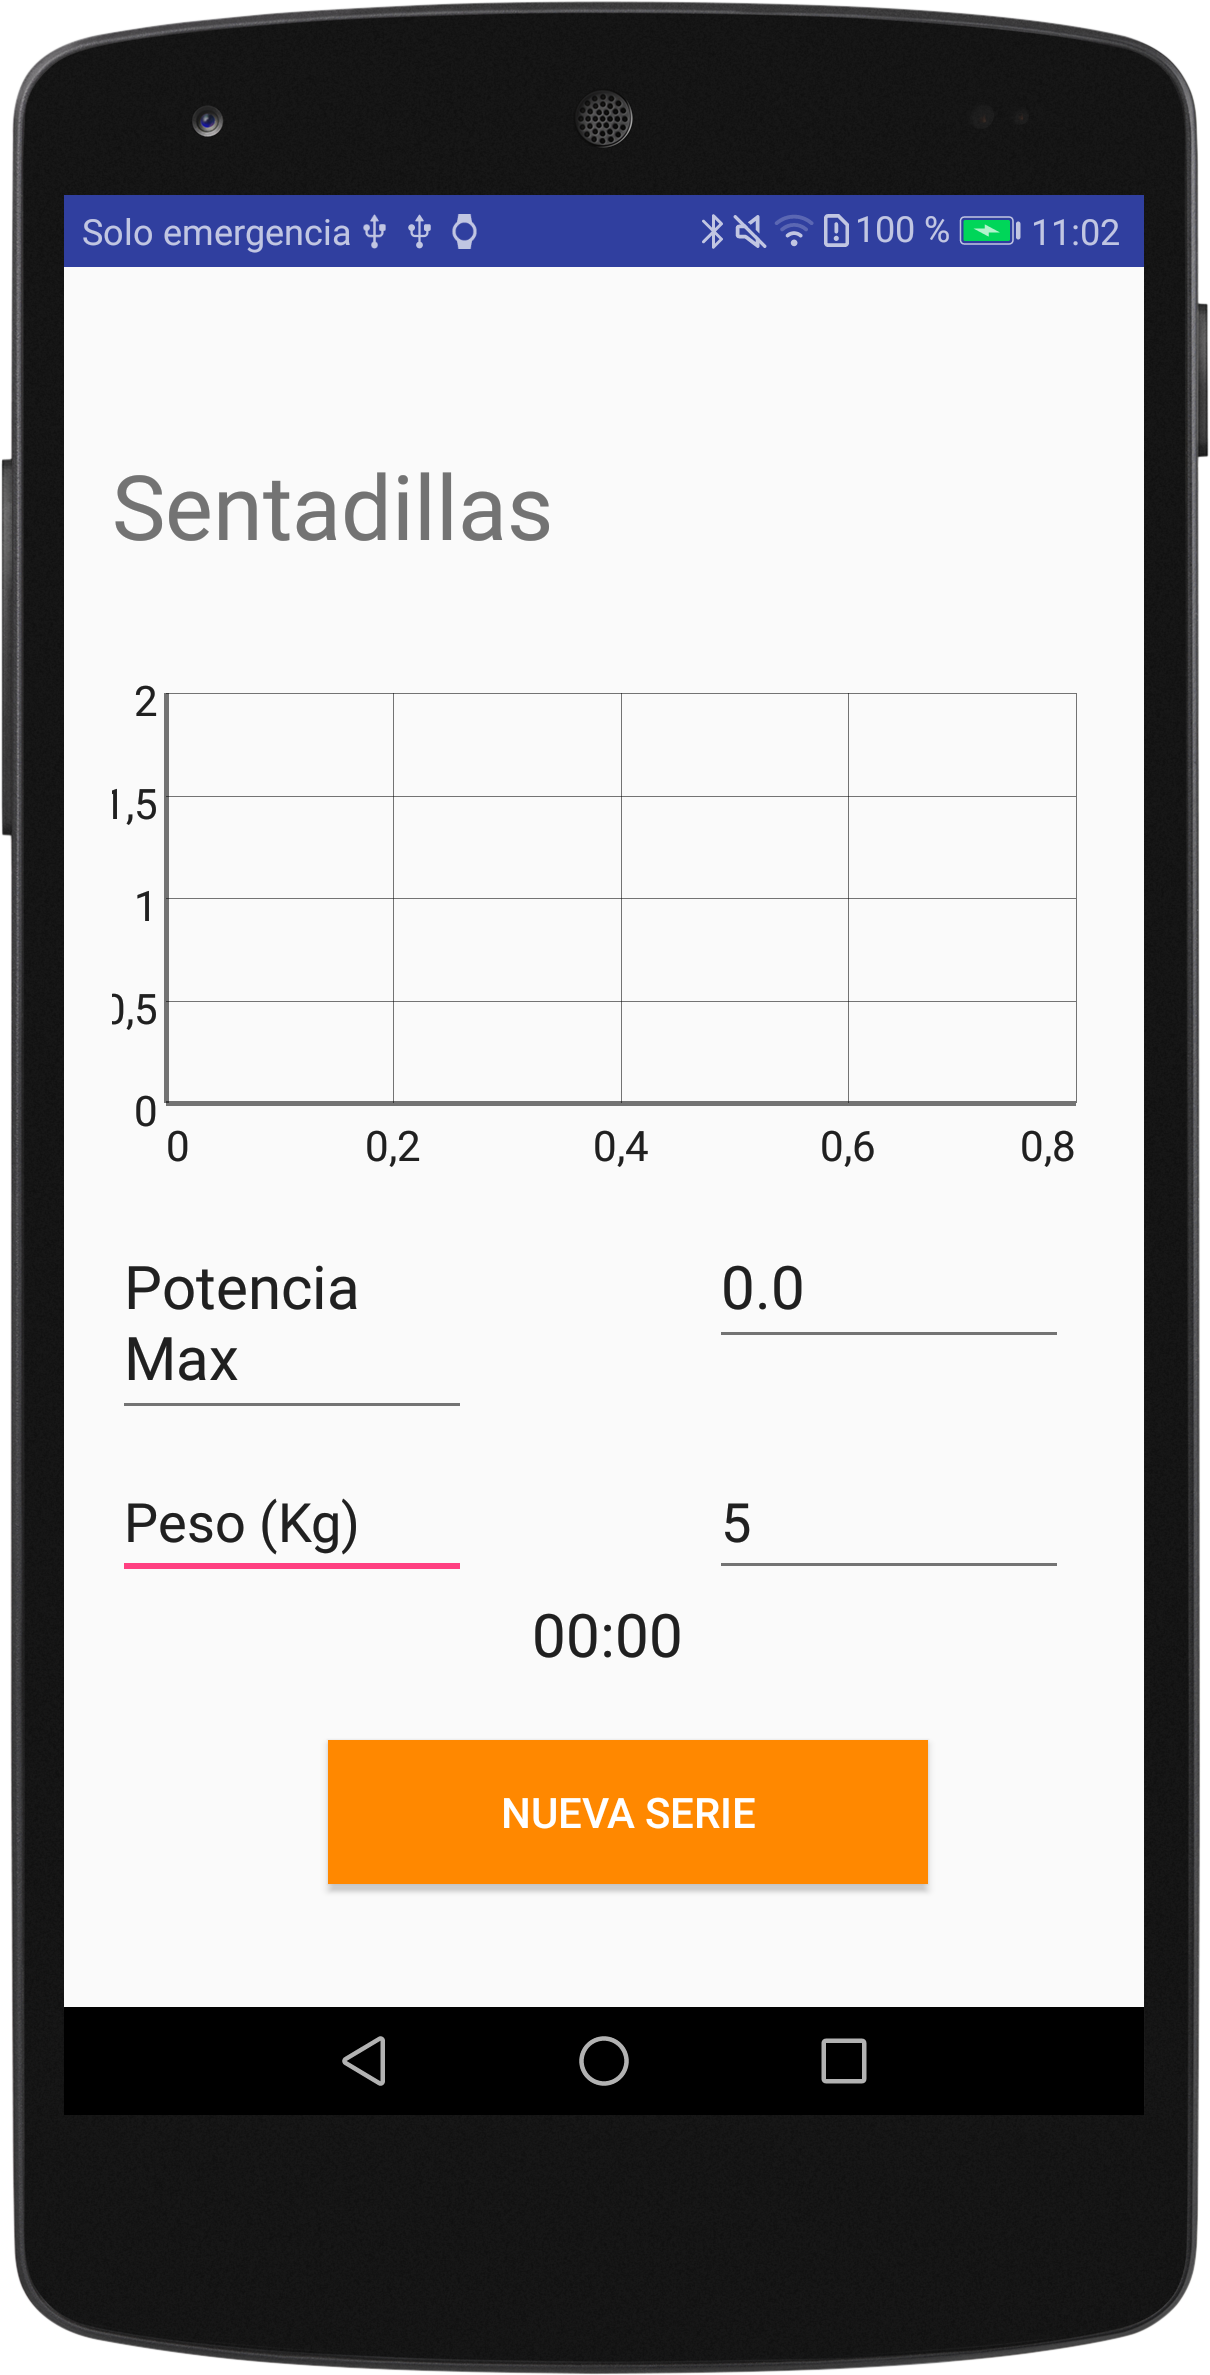
\includegraphics[scale=0.10]{imagenes/m6.png}
	\caption{Vista inicial ejercicio móvil}
	\label{Vista inicial ejercicio movil}
\end{figure}

\begin{figure}[H]
	\centering
	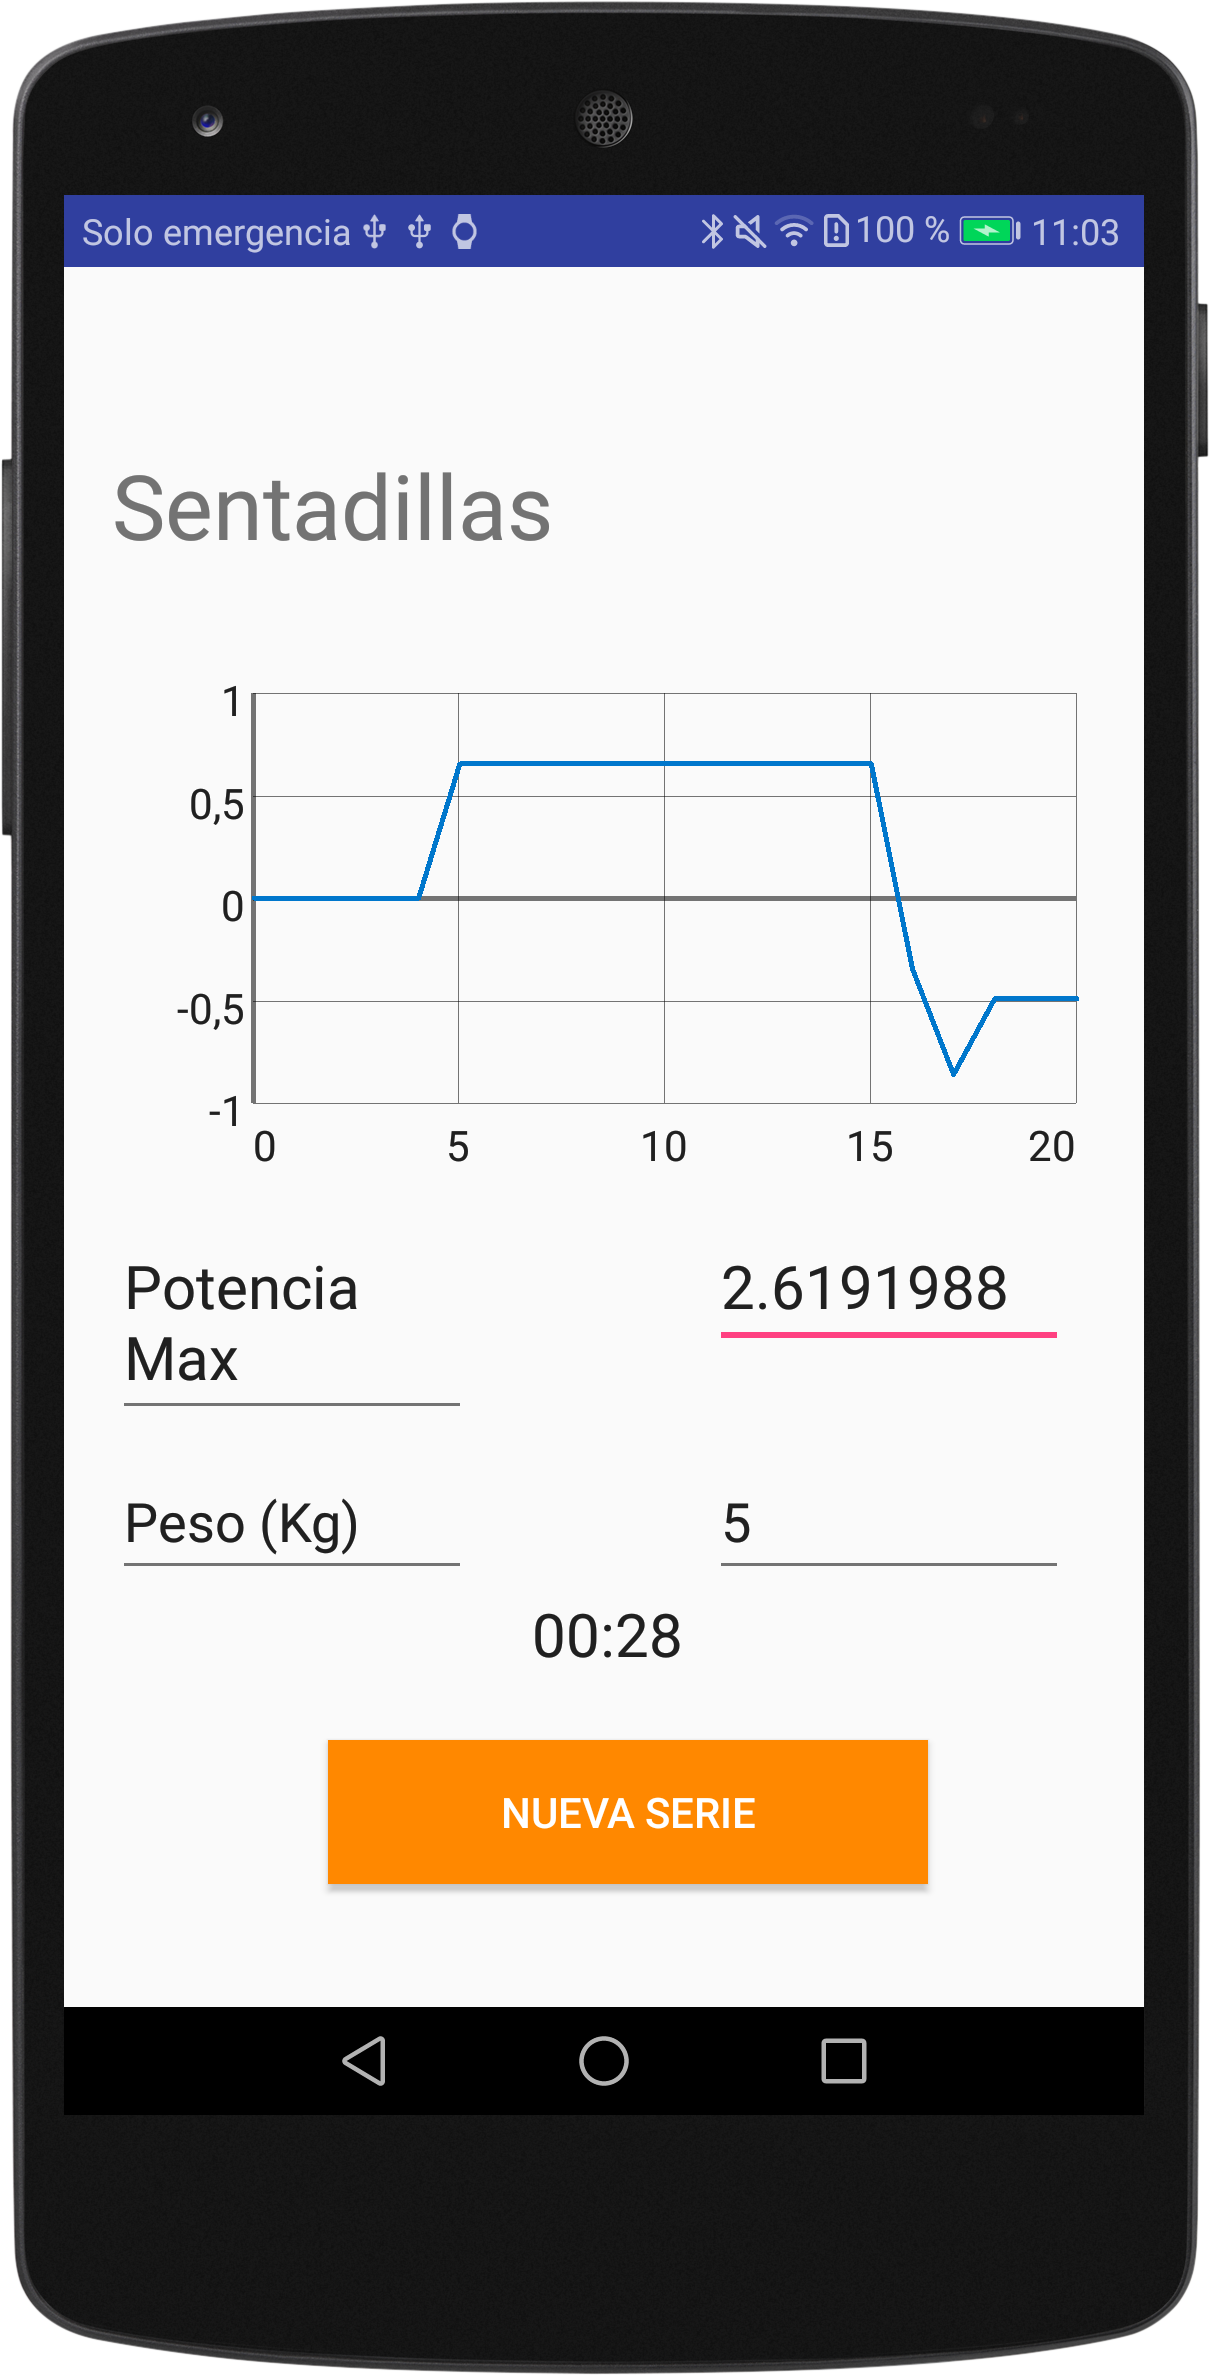
\includegraphics[scale=0.10]{imagenes/m7.png}
	\caption{Vista realización ejercicio móvil}
	\label{Vista realización ejercicio movil}
\end{figure}
